%%% CHEP 2019 protoDUNE-SP DQM evolution paper

%%%\documentclass[option]{webofc}
%%% "twocolumn" for typesetting an article in two columns format (default one column)


\documentclass{webofc}
\usepackage[varg]{txfonts}   % Web of Conferences font

%
% Put here some packages required or/and some personnal commands
%

\usepackage{xspace}
\usepackage{tabularx}

\newcommand{\pd}{protoDUNE\xspace}
\newcommand{\filesize}{8\,GB\xspace}

%%%%%%%%%%%%%%%%%%%%%%%%%%%% BEGIN %%%%%%%%%%%%%%%%%%%%%%%%%%%%%%%

\begin{document}
%
\title{Evolution of the Data Quality Monitoring and Prompt Processing System in the protoDUNE-SP experiment}


\author{
\firstname{Maxim} 
\lastname{Potekhin}\inst{1}\fnsep\thanks{\email{potekhin@bnl.gov}}, \it{on behalf of the DUNE Collaboration}
}

\institute{Brookhaven National Laboratory, Upton, NY11973, USA}


\abstract{
The DUNE Collaboration currently operates
an experimental program based at CERN which includes a beam test and an extended
cosmic ray run of two large-scale prototypes of the massive Liquid Argon Time
Projection Chamber for the DUNE Far Detector. The volume of data collected by the single-phase prototype
(protoDUNE-SP) amounts to $\sim$3PB and the sustained rate
of data sent to mass storage is O(100)\,MB/s.  Data Quality Monitoring
was implemented by directing a fraction of the data stream
to the protoDUNE Prompt Processing System (p3s) which is optimized
for continuous low-latency calculation of the vital detector metrics and various graphics
including event displays. It served a crucial role throughout the life cycle of the
experiment. We present our experience in leveraging the CERN computing
environment and operating the system over an extended period of time, while
adapting to evolving requirements and computing platform.
}
%
\maketitle
%
\section{Introduction}
\label{sec:intro}

The aim of the \pd-SP experiment  \cite{spanu} is a detailed study of a large-scale prototype
of the massive 10kt single-phase Liquid Argon Time Projection Chamber (LArTPC) to be used
in the DUNE experiment  \cite{cdrVol1, cdrVol4}. The experiment took test beam data in
2018 and cosmic ray data throughout 2019. The nature of the experiment requires a versatile
Data Quality Monitoring (DQM) system capable of performing complex calculations on
a few minutes time scale as well as preserving the results (inluding various types of graphics
and tabulated data) in an easily accessible form and over an extended period of time.
In order to support this capability a \textit{protoDUNE prompt processing system} (p3s)
was designed, deployed and operated for 3 years \cite{eps}. Its design proved flexible
enough to quickly adapt to different hardware platforms and computational payloads.

\section{System Design}
\label{sec:outline}

A predefined (and configurable) fraction of the data written to a local buffer
by the  \pd-SP Data Acquisition (DAQ) system is  transferred to a dedicated space
in the  CERN EOS disk storage  \cite{castoreos,eos_role} by an instance of the ``Fermi-FTS''
data handling system \cite{fts}. Arrival of new data is detected by an automated process
polling the corresponsing directory in EOS and triggers creation of jobs records in the
p3s database, forming a queue. The p3s brokerage module then matches these jobs records
to available pilot jobs (running asynchronously on the worker nodes within the designated
resource) and provides the pilot with information necessary to actuate the ``payload job'' (e.g.\,as via a URL
pointing to a script and a set of parameters). Monitoring information about execution
of the payloads is presented to the user in the p3s Web UI.
Job outputs are automatically catalogued in the database and are made available
to the users via a Web interface through a set of selectors and menus.
The following is a summary  of the \pd-SP
prompt processing/DQM system design features\cite{chep18}:
\begin{itemize}

\item A high degree of automation and a data-driven workflow
%: creation of various computational payloads is triggered by arrival of new data

\item A complete decoupling of the DQM and the DAQ systems, which allows
for stable and reliable operation of the latter while being able to make frequent updates to the
DQM code and adding new types of software modules (``payloads'') when necessary
%, as well as adjusting operating parameters of the system

\item A pilot-based framework inspired by PanDA and Dirac \cite{panda,dirac}
which minimizes the latency of job submission and provides a layer of abstraction
of the computing resources; a Web application coordinates the operation of ``pilot jobs''
which in turn manage the execution of the ``payload jobs''

\item Separation of the workload management functionality  of p3s  from
indexing and navigation of the content created by the DQM  jobs (a separate ``content service''),
which provides a clean interface and optimal end-user experience
% ; such separation is achieved by creating two distinct Web services

\item Utilization of an indistry-standard Django Web application framework  \cite{django},
with the applications hosted by Apache Web servers while utilzing the PostgreSQL database
back-end

\item Self-describing DQM data which allows automatic and consistent generation of Web pages
by the content service for each type of DQM applications without changes to the server code
 this is achieved by the requirement that DQM jobs produce a peice of metadata (a set of JSON files)
which completely describes their output dataset and the logic of its navigation

\end{itemize}
\noindent
A conceptual diagram of the prompt processing and DQM system components
is presented in figure~\ref{dqm-diagram}.

\begin{figure}[h]
\centering
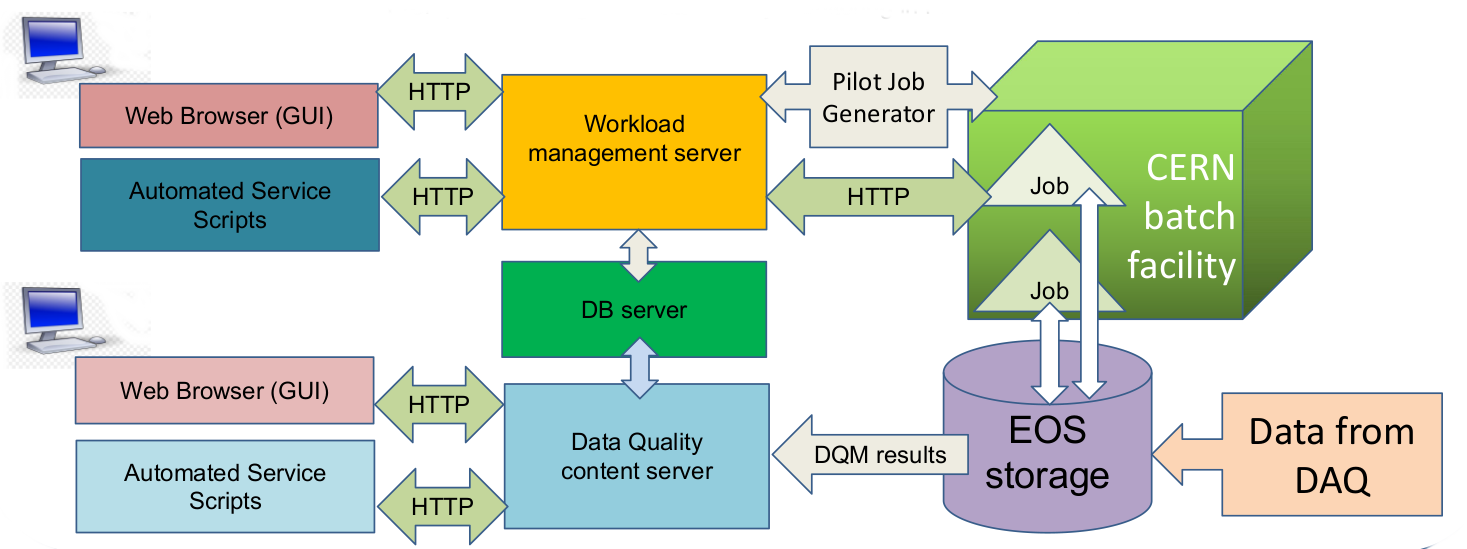
\includegraphics[width=0.9\textwidth,clip]{figures/dqm-p3s-diagram.png}
\caption{The protoDUNE-SP prompt processing and DQM systems}
\label{dqm-diagram}
\end{figure}

%%%%%%%%%%%%%%%%%%%%%%%%%%%%%%%%%%%%%%%%%
\section{System Evolution}

\subsection{The Hardware Platform}
\label{sec:hardware}

The p3s pilot-based framework provides substabtial flexibility in accessing and
managing the available computing resource. Generation of pilot jobs is external
to the core system itself and thus can be easily adapted to a particular resource.
One basic requirement is that the pilot jobs running on the worker nodes have
HTTP access to the p3s server. The first (test) instance of p3s deployed
on an \textit{ad hoc} colleciton of local machines used the parallel remote shell
(pdsh) to manage the population of pilot jobs running on the worker nodes.
The next deployment was on a hardware cluster provided by the CERN
Neutrino Platform organization \cite{platform} consisting of a few dozen
worker nodes configured as a HTCondor cluster, and the pilots were managed
by scripts utilizing the HTCondor batch system tools. Web services were deployed
on two nodes which were part of the same cluster.



%For tables use syntax in table~\ref{tab-1}.
%\begin{table}
%\centering
%\caption{Please write your table caption here}
%\label{tab-1}       % Give a unique label
%% For LaTeX tables you can use
%\begin{tabular}{lll}
%\hline
%first & second & third  \\\hline
%number & number & number \\
%number & number & number \\\hline
%\end{tabular}
%% Or use
%\vspace*{5cm}  % with the correct table height
%\end{table}

\begin{thebibliography}{99}

\bibitem{spanu}
M. Spanu
\emph{The status and results from ProtoDUNE Single Phase}
IOP Conf. Series: Journal of Physics: Conf. Series \textbf{1312} (2019) 012003

\bibitem{cdrVol1}
R. Acciarri et al.
\emph{Long-Baseline Neutrino Facility (LBNF) and Deep Underground Neutrino Experiment (DUNE) Conceptual Design Report Volume 1: The LBNF and DUNE Projects}.\\ ~e-Print: arXiv:\textbf{1601.05471}


\bibitem{cdrVol4}
R. Acciarri et al.
\emph{Long-Baseline Neutrino Facility (LBNF) and Deep Underground Neutrino Experiment (DUNE) Conceptual Design Report, Volume 4: The DUNE Detectors at LBNF}.\\~e-Print: arXiv:\textbf{1601.02984}

\bibitem{eps} M.Potekhin et al. \emph{The protoDUNE-SP experiment and its prompt
processing system}. Proceedings of Science (EPS-HEP2017) 513


\bibitem{castoreos}
L. Mascetti et al. \emph{Disk storage at CERN.~J. Phys.: Conf. Series.} Vol.\textbf{664}. IOP Publishing, 2015,
doi:10.1088/1742-6596/664/4/042035

\bibitem{eos_role}
S. Fuess et al. \emph{Design of the protoDUNE raw data management
infrastructure.~J. Phys.: Conf. Series.} Vol.\textbf{898}. IOP Publishing, 2017,
doi:10.1088/1742-6596/898/6/062036

\bibitem{fts}
A. Norman \emph{The Fermilab File Transfer System}.~e-Print: FNAL CD-DocDB-5412

\bibitem{chep18} M. Potekhin et al. \emph{The Prompt Processing System
and Data Quality Monitoring in the protoDUNE-SP Experiment}
EPJ Web of Conferences \textbf{214}, 01026 (2019)

\bibitem{panda}
T. Maeno et al. \emph{Overview of ATLAS PanDA Workload Management.~J. Phys.: Conf. Series.} Vol.\textbf{331}. IOP Publishing, 2011,
doi:10.1088/1742-6596/331/7/072024


\bibitem{dirac}
A. Casajus et al.  \emph{DIRAC Pilot Framework and the DIRAC
Workload Management System.~J. Phys.: Conf. Series.} Vol.\textbf{219}. IOP Publishing, 2010,
doi:10.1088/1742-6596/219/6/062049


\bibitem{django}
N. George \emph{Mastering Django: Core. The Complete Guide to Django 1.8 LTS}~ GNW Independent Publishing, ISBN: 099461683X

\bibitem{platform} F. Pietropaolo \emph{Review of Liquid-Argon Detectors Development at the CERN
Neutrino Platform}
IOP Conf. Series:  Journal of Physics: Conf. Series \textbf{888} (2017) 012038


\end{thebibliography}




\end{document}

% end of file template.tex

<div id='footer'><table width='100%'><tr><td class='right'><a href='http://fusioninventory.org/'><span class='copyright'>FusionInventory 9.1+1.0 | copyleft <img src='/glpi/plugins/fusioninventory/pics/copyleft.png'/>  2010-2016 by FusionInventory Team</span></a></td></tr></table></div>